%! TEX root = main.tex

\chapter{1D Continuous Systems}

Discrete models (masses, springs, dampers) capture many key ideas in musical acoustics, but real vibrating objects are spatially extended. A string, a bar or a plate cannot be described by a finite set of generalized coordinates unless one performs a truncation: they are continuous systems with (in principle) infinitely many degrees of freedom. The dynamics are therefore governed by partial differential equations (PDEs) and the observed motion results from the interplay between wave propagation, reflections at terminations, modal standing-wave patterns and dissipation. In this chapter, we introduce the basic 1D building blocks: transverse waves in strings (traveling and standing waves, plucked/struck/bowed excitation, driven response and impedance, boundary conditions, damping) and then longitudinal, bending and torsional waves in bars and stiff strings.

\section{Transverse Waves in an Ideal String}

Consider a taut string with uniform tension \( T \) and linear mass density \( \mu \) (\si{\kilo\gram\per\meter}). Let \( y(x,t) \) denote the transverse displacement from the equilibrium line. In order for oscillations to occur, a restoring force must act on the displaced string; in a string, this restoring action is provided by the vertical component of the tension at the ends of a small element. 

\subsection{Derivation of the Wave Equation}

\begin{figure}[!htb]
    \centering
    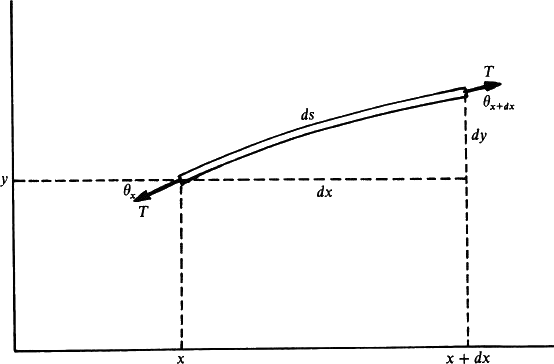
\includegraphics[width=0.65\linewidth]{00_Images/02_chapter/01.png}
    \caption{Forces on a differential string element under tension \(T\)}
    \label{fig:stringelement}
\end{figure}

Take a short string segment between \( x \) and \( x + dx \). The geometry and the force balance on the differential element are sketched in figure \ref{fig:stringelement}. The vertical components of the tension at the two ends are \( (T\sin\theta)_x \) and \( (T\sin\theta)_{x + dx} \). The net vertical force on the segment is therefore
\[
dF_y = (T\sin\theta)_{x + dx} - (T\sin\theta)_x
    = \frac{\partial(T\sin\theta)}{\partial x}dx
\]
For small transverse displacements, the slope is small and one may approximate
\[
\sin\theta \simeq \tan\theta = \frac{\partial y}{\partial x}
\]
so that
\[
dF_y = T\frac{\partial^2 y}{\partial x^2}dx
\]
Applying Newton's second law to the same element,
\[
dF_y = (\mu ds)\frac{\partial^2 y}{\partial t^2}
\]
and for small displacements \( ds\simeq dx \). Hence,
\[
T\frac{\partial^2 y}{\partial x^2}dx = \mu dx\frac{\partial^2 y}{\partial t^2}
\qquad\Longrightarrow\qquad
\frac{\partial^2 y}{\partial t^2} = c^2\frac{\partial^2 y}{\partial x^2}
\]
where the transverse wave speed is
\[
c = \sqrt{\frac{T}{\mu}}
\]
This is the one-dimensional wave equation for an ideal string (uniform tension, small slopes, no losses).

\subsection{Traveling-Wave Solution and Boundary Conditions}

The general solution of the wave equation can be written as the superposition of two traveling waves,
\[
y(x,t) = f_1(ct-x) + f_2(ct + x)
\]
where \( f_1 \) travels towards increasing \( x \) and \( f_2 \) travels towards decreasing \( x \), both with speed \( c \).
To determine the specific functions \( f_1 \) and \( f_2 \), two types of constraints are required:

\begin{itemize}
\item Initial conditions: the displacement \( y(x,0) \) and velocity \( \partial y/\partial t(x,0) \) must match the initial state produced by the excitation.
\item Boundary conditions: for a finite string, conditions must be satisfied at the endpoints (values of \( y \) or its spatial derivative).
\end{itemize}

Two idealized endpoint conditions are especially important. Assuming the end is located at \( x = 0 \):

\begin{itemize}
\item Fixed end: \( y(0,t) = 0 \). Then
\[
f_1(ct) + f_2(ct) = 0
\qquad\Longrightarrow\qquad
f_1(ct) = -f_2(ct)
\]
the reflected traveling wave is inverted in sign.
\item Free end: no transverse force can be exerted; hence \( \partial y/\partial x(0,t) = 0 \). Since
\[
\frac{\partial y}{\partial x} = -f_1'(ct-x) + f_2'(ct + x)
\]
at \( x = 0 \) one obtains
\[
-f_1'(ct) + f_2'(ct) = 0
\qquad\Longrightarrow\qquad
f_2'(ct) = f_1'(ct)
\]
Under the usual assumption of no energy creation at the boundary, this implies \( f_1(ct) = f_2(ct) \): the reflected wave is non-inverted.
\end{itemize}

\subsection{Harmonic Waves and Wavenumber}

Any complex waveform can be decomposed into (possibly infinitely many) sinusoidal components. Consider a single harmonic component at temporal angular frequency \( \omega \). A general real traveling-wave representation is
\[
y(x,t) = A\sin(\omega t-kx) + B\cos(\omega t-kx) + C\sin(\omega t + kx) + D\cos(\omega t + kx)
\]
where the wavenumber \( k \) is
\[
k = \frac{\omega}{c} = \frac{2\pi}{\lambda}
\]
and \( \lambda \) is the wavelength. It is often convenient to use the complex form,
\[
\widetilde{y}(x,t) = \widetilde{A}e^{j(\omega t-kx)} + \widetilde{B}e^{j(\omega t + kx)},
\qquad
y(x,t) = \Re\{\widetilde{y}(x,t)\}
\]
The arbitrary constants (either \( A,B,C,D \) or \( \widetilde{A},\widetilde{B} \) ) are determined by imposing initial and boundary conditions.

\subsection{Standing Waves and Normal Modes of a Fixed String}

Consider a string of length \( L \) fixed at both ends (\( x = 0 \) and \( x = L \)). The fixed-end conditions require
\[
y(0,t) = 0,\qquad y(L,t) = 0
\]
Imposing \( y(0,t) = 0 \) forces the left- and right-traveling components to combine into a standing wave form, which can be written as
\[
y(x,t) = 2\sin(kx)\left[A\cos(\omega t)-B\sin(\omega t)\right]
\]
Imposing the second boundary condition \( y(L,t) = 0 \) yields
\[
\sin(kL) = 0
\qquad\Longrightarrow\qquad
kL = n\pi,\quad n\in\mathbb{N}
\]
Using \( k = \omega/c \), the admissible (angular) frequencies are
\[
\omega_n = \frac{n\pi c}{L},
\qquad
k_n = \frac{n\pi}{L}
\]
The corresponding standing-wave patterns are the normal modes of the fixed string and a modal expansion of the motion may be written as
\[
y(x,t) = \sum_{n = 1}^{\infty}\left(A_n\sin(\omega_n t) + B_n\cos(\omega_n t)\right)\sin(k_n x)
\]
The constants \( A_n \) and \( B_n \) are set by the initial conditions, which in practice depend on the excitation mechanism (plucked, struck, bowed or externally driven).

\subsection{String Excitation Mechanisms: Plucked, Struck and Bowed}

The wave equation and its normal modes describe the admissible motions of an ideal string, but the actual vibration observed in an instrument depends crucially on how the motion is initiated and sustained. In this part we summarize three archetypal excitation mechanisms-plucking, striking and bowing-and show how they shape the modal amplitudes and the resulting spectrum.

\subsubsection{Plucked Strings: Modal Coefficients and Missing Harmonics}

When a string is plucked, the initial triangular displacement can be expanded in normal modes. Figure \ref{fig:pluckmodes} illustrates the modal distribution for a string plucked at midspan: by symmetry, even modes have vanishing participation while odd modes dominate the response.

\begin{figure}[!htb]
    \centering
    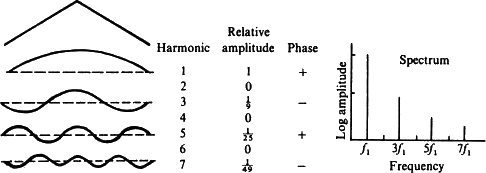
\includegraphics[width=0.9\linewidth]{00_Images/02_chapter/02.png}
    \caption{Modal participation for a string plucked at midspan}
    \label{fig:pluckmodes}
\end{figure}

For a string of length \( L \) fixed at both ends, the displacement can be expanded in normal modes as
\[
y(x,t) = \sum_{n = 1}^{\infty}\left[A_n\sin(\omega_n t) + B_n\cos(\omega_n t)\right]\sin\left(\frac{n\pi x}{L}\right),
\qquad
\omega_n = \frac{n\pi c}{L}
\]
The coefficients are determined by the initial conditions \( y(x,0) \) and \( \dot{y}(x,0) \) through orthogonality:
\[
A_n = \frac{2}{\omega_n L}\int_{0}^{L}\dot{y}(x,0)\sin\left(\frac{n\pi x}{L}\right)dx,
\qquad
B_n = \frac{2}{L}\int_{0}^{L}y(x,0)\sin\left(\frac{n\pi x}{L}\right)dx
\]
For an ideal pluck released from rest, one has \( \dot{y}(x,0) = 0 \), hence \( A_n = 0 \) and the spectrum is entirely determined by \( B_n \).

\paragraph{Pluck at the midpoint} Assume a triangular initial shape with maximum displacement \( h \) at \( x = L/2 \). The resulting coefficients take the form
\[
B_n = \frac{8h}{\pi^2 n^2}\sin\left(\frac{n\pi}{2}\right)
\]
Therefore all even modes are absent (since \( \sin(n\pi/2) = 0 \) for even \( n \) ), while the odd harmonics alternate in sign because \( \sin(n\pi/2) = \pm 1 \). This selection rule is a direct consequence of symmetry: even modes have a node at the midpoint and cannot reproduce a midpoint maximum at \( t = 0 \).

\paragraph{Pluck at a fraction of the length} Let the string be plucked at \( x = L/5 \) and released from rest with a triangular initial displacement of height \( h \). Then
\[
B_n = \frac{25h}{2\pi^2 n^2}\sin\left(\frac{n\pi}{5}\right),
\qquad
A_n = 0
\]
The factor \( \sin(n\pi/5) \) implies \( B_n = 0 \) for \( n = 5,10,15,\dots \): when the pluck point is at \( x = L/g \) with \( g\in\mathbb{N} \), the modes \( g,2g,3g,\dots \) are absent. In the time domain, the initial triangular shape may be interpreted as two sharp bends that propagate in opposite directions and reflect at the ends, generating the familiar periodic motion of a plucked string. 

\begin{figure}[!htb]
    \centering
    \subfloat[Evolution and the resulting boundary force]{
        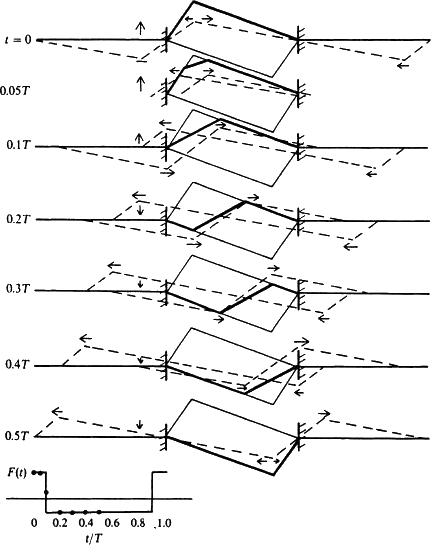
\includegraphics[width=0.45\linewidth]{00_Images/02_chapter/03.png}
    }
    \hfill
    \subfloat[Spectrum of the modes]{
        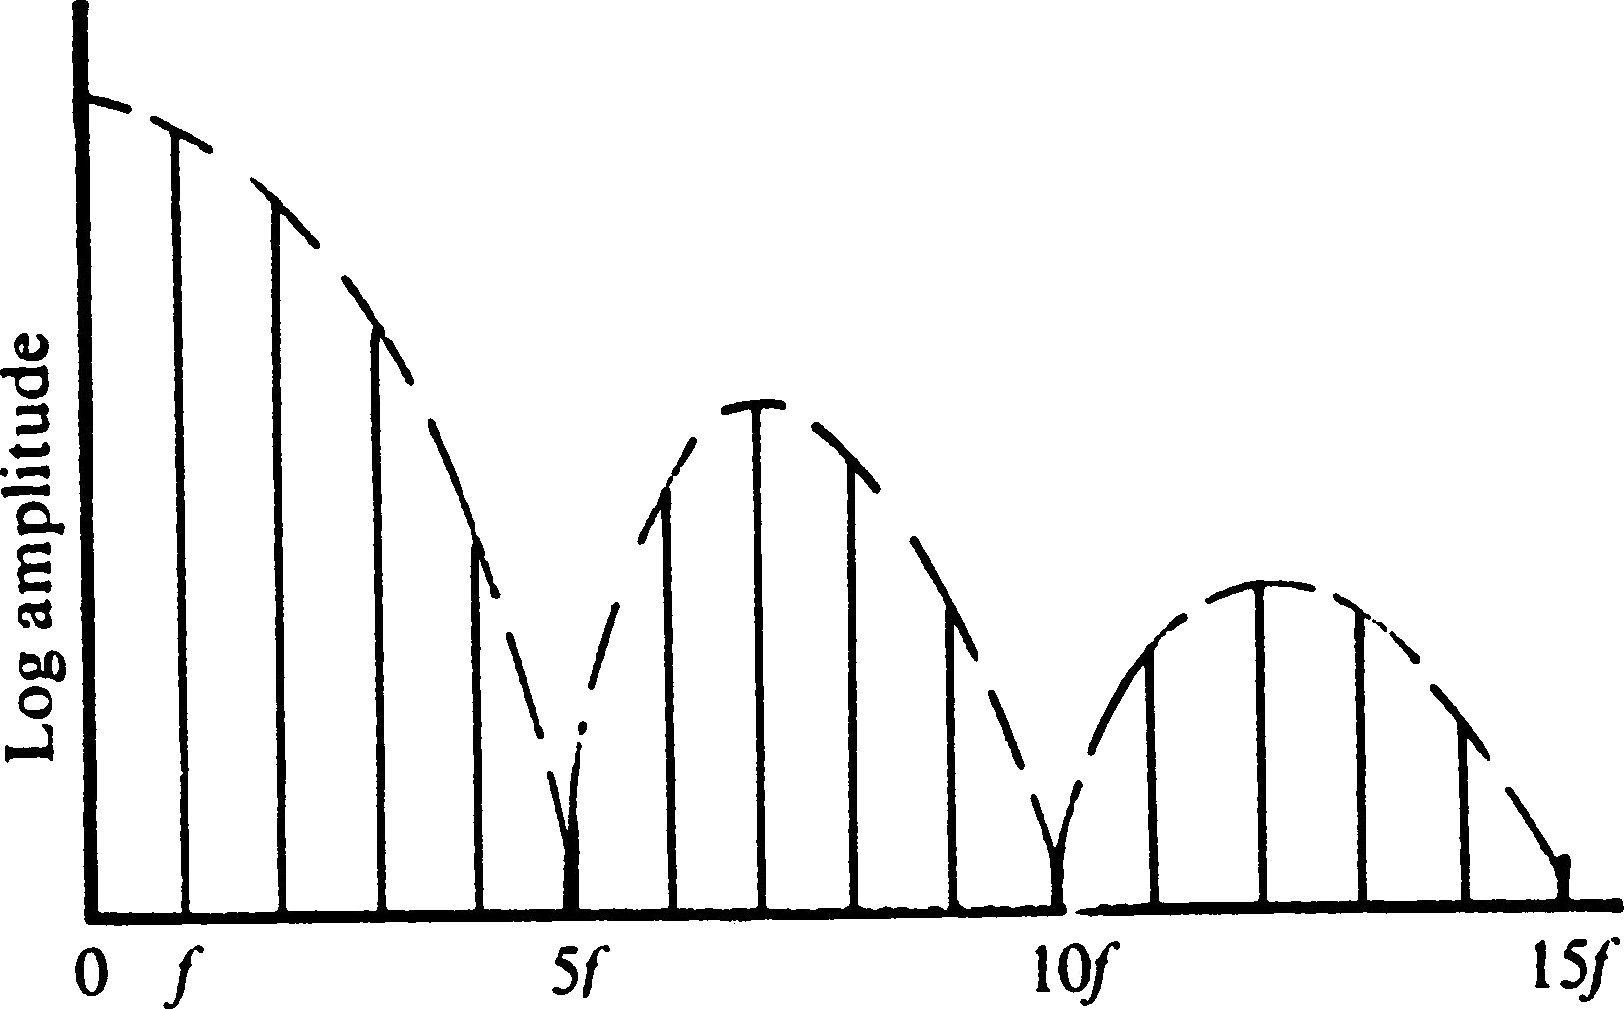
\includegraphics[width=0.45\linewidth]{00_Images/02_chapter/04.png}
    }
    \caption{Results for a string plucked at one-fifth of its total length}
    \label{fig:pluckevolution}
\end{figure}

\subsubsection{Struck Strings: Hammer Interaction and Spectral Envelope}

In a struck string, the excitation is mediated by a hammer of finite mass \( M \) impacting the string at \( x = x_0 \) with initial velocity \( V \). As time increases, the disturbance spreads along the string: after a time \( t \) the portion of string involved in the motion has length \( 2ct \) and mass \( 2\mu ct \). As this effective moving mass becomes comparable with \( M \), the hammer is progressively slowed down. At the contact point, the force exerted by the hammer must be balanced by the restoring force associated with the string tension. This can be expressed by writing Newton's law for the hammer in terms of the discontinuity of the string slope at the impact point,
\[
M\frac{\partial^2 y}{\partial t^2}(x_0,t) = T\Delta\left(\frac{\partial y}{\partial x}\right)
\]
where \( \Delta(\partial y/\partial x) \) denotes the jump in slope across \( x_0 \). Solving this interaction problem (before any reflected waves return to the contact point) yields an exponentially decaying contact velocity
\[
v(x_0,t) = V e^{-t/\tau},
\qquad
\tau = \frac{Mc}{2T}
\]
and the corresponding contact displacement
\[
y(x_0,t) = V\tau\left(1-e^{-t/\tau}\right)
\]
For a finite string, reflections from the endpoints eventually return to \( x_0 \) and can throw the hammer off the string before it comes fully to rest; after separation, the string vibrates freely in its normal modes.

\paragraph{Spectral consequences} Compared with plucking (where modal amplitudes typically scale as \( 1/n^2 \) ), striking produces a much richer high-frequency content. In the limit \( M\ll M_s \) (string mass \( M_s \) ), the displacement spectrum exhibits dips to zero at harmonic numbers that are multiples of \( 1/\beta \) when the string is struck at a fraction \( \beta \) of its length, while remaining otherwise relatively flat. If \( M \) is small but not negligible, the spectrum is approximately constant up to a mode number
\[
n_m \simeq 0.73\frac{M_s}{M}
\]
and above \( n_m \) it falls off as \( 1/n \), i.e. much more slowly than for plucking. The traveling velocity pulses that initiate this response are illustrated in figure \ref{fig:struckpulses}.

\begin{figure}[!htb]
    \centering
    
\includegraphics[width=0.9\linewidth]{00_Images/02_chapter/05.png}
    \caption{Velocity pulses generated by striking a string}
    \label{fig:struckpulses}
\end{figure}

\subsubsection{Bowed Strings: Helmholtz Motion and Stick-Slip Energy Input}

The bowed string is not merely an initial-value problem: the bow continuously injects energy into the string through friction at the contact point. The ideal periodic motion of a bowed string is known as Helmholtz motion. Kinematically, the string waveform is approximately triangular, with a single sharp bend (a traveling ``corner'') that runs back and forth along the string. At a fixed observation point, the velocity waveform alternates between two values, reflecting the alternation between two dynamical regimes. The characteristic waveform and the associated stick-slip cycle are summarized in figure \ref{fig:helmholtz_stickslip}.

\begin{figure}[!htb]
    \centering
    \subfloat[Helmholtz waveform and velocity at different positions]{
        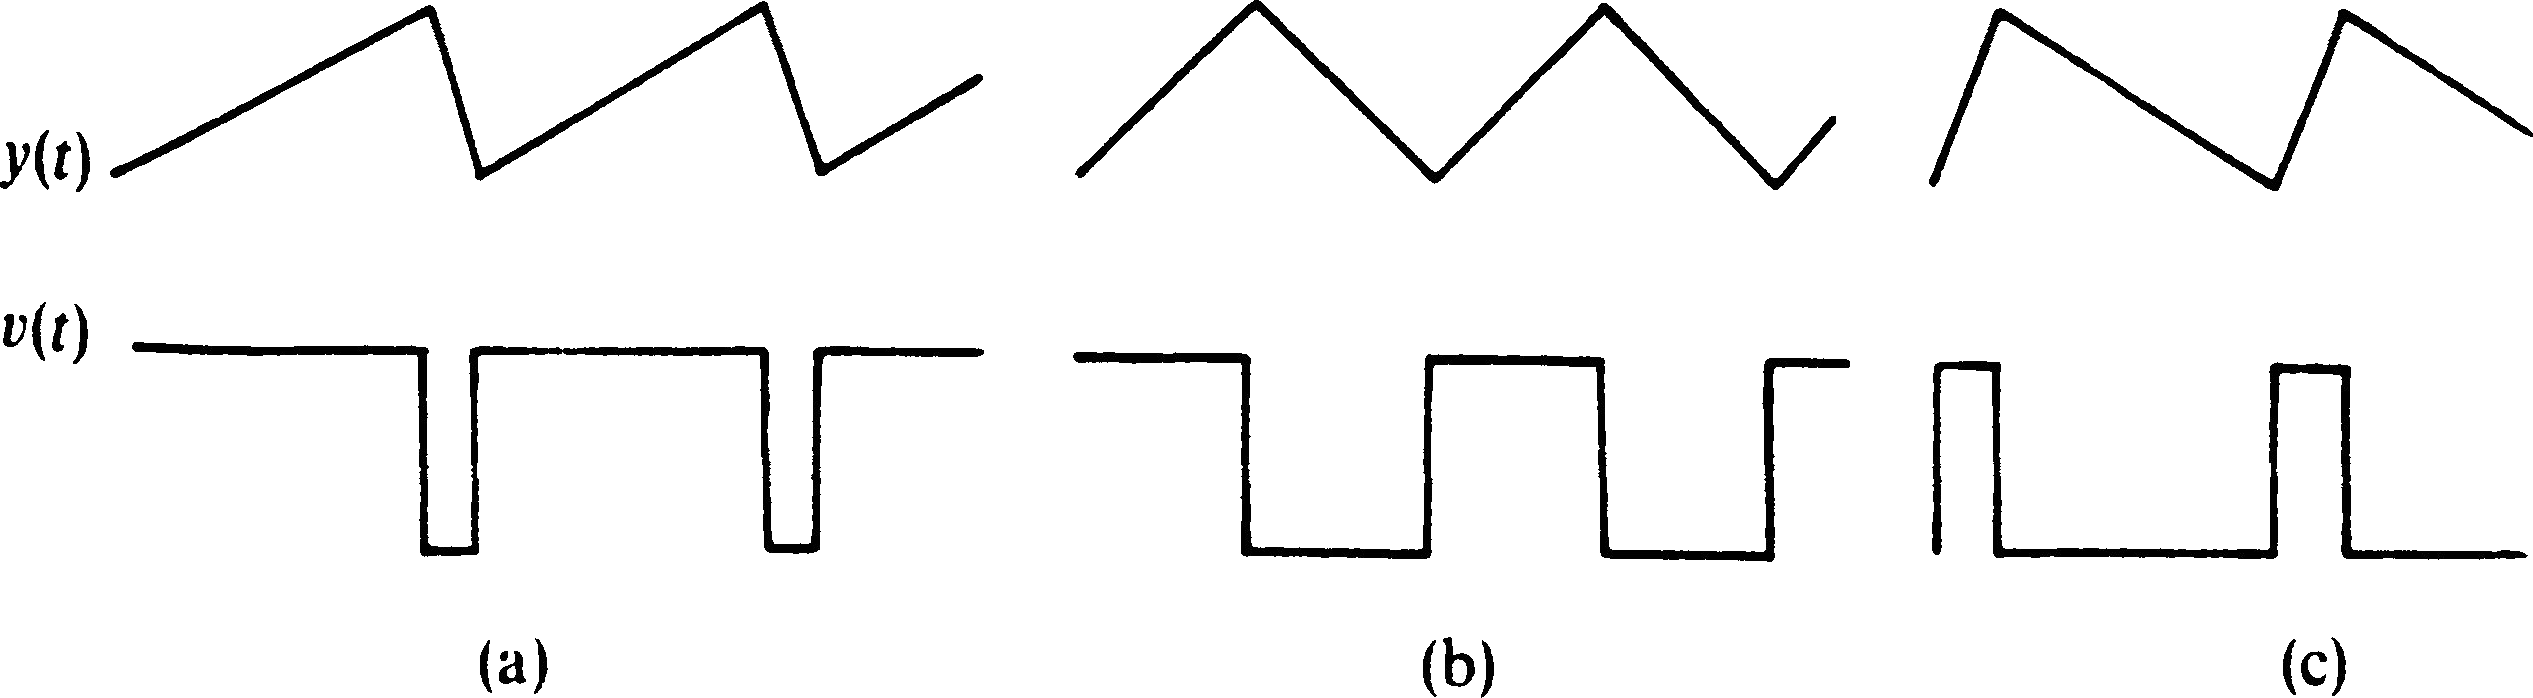
\includegraphics[width=0.48\linewidth]{00_Images/02_chapter/06.png}
    }\hfill
    \subfloat[Stick-slip cycle at the bowing point]{
        
\includegraphics[width=0.48\linewidth]{00_Images/02_chapter/07.png}
    }
    \caption{Helmholtz motion in a bowed string and the corresponding stick-slip mechanism}
    \label{fig:helmholtz_stickslip}
\end{figure}

\paragraph{Stick-slip mechanism} During part of the cycle the bow hair drags the string (stick phase): bow and string move in the same direction and static friction dominates. When the traveling bend arrives at the bowing point, the string suddenly releases (slip phase): bow and string move in opposite directions and dynamic friction dominates. Since the frictional force is higher during the stick phase, the net energy transfer over a full cycle is from the bow to the string, compensating internal and radiation losses and sustaining steady oscillation.

\paragraph{Comparison with plucking} A plucked string can be interpreted as two counter propagating bends (two traveling discontinuities), while the ideal bowed string exhibits a single traveling bend. This difference is reflected in the time waveform and in the harmonic content: the near piecewise-linear displacement and piecewise-constant velocity of Helmholtz motion naturally support a strong harmonic series, consistent with the bright timbre of bowed-string instruments.

\subsection{Input Impedance of a String}

\paragraph{Semi-Infinite String} Consider a string driven at \( x = 0 \) by a harmonic force
\[
e_f(t) = F e^{j\omega t}
\]
Assume first an infinitely long string, so that no reflected wave is present: only a forward-traveling wave propagating towards increasing \( x \) can exist,
\[
y_e(x,t) = A e^{j(\omega t-kx)}
\]
At the driving point, the applied force must be balanced by the vertical component of the string tension. Under small-slope assumptions,
\[
F e^{j\omega t} = -T\left.\frac{\partial y_e}{\partial x}\right|_{x = 0}
\]
Since \( \partial y_e/\partial x = -jkA e^{j(\omega t-kx)} \), at \( x = 0 \) this gives
\[
F e^{j\omega t} = jkT A e^{j\omega t}
\qquad\Longrightarrow\qquad
A = -j\frac{F}{kT}
\]
The transverse velocity follows from time differentiation:
\[
u_e(x,t) = \frac{\partial y_e}{\partial t}
 = j\omega A e^{j(\omega t-kx)}
 = \frac{F\omega}{kT}e^{j(\omega t-kx)}
\]
The input impedance (driving-point impedance) is defined as the ratio of force to velocity at the driving point,
\[
Z_{\mathrm{in}} = \left.\frac{\text{Force}}{\text{Velocity}}\right|_{x = 0}
 = \frac{F e^{j\omega t}}{u_e(0,t)}
 = \frac{kT}{\omega}
 = \frac{T}{c},
\qquad c = \frac{\omega}{k}
\]
Hence, the input impedance of an infinite string is purely resistive and constant: it does not depend on frequency or on the position where the string is driven.

\paragraph{Finite String} Now consider a finite string of length \( L \), fixed at the far end:
\[
y_e(L,t) = 0
\]
Because of reflection at \( x = L \), the motion is a superposition of forward and backward traveling waves,
\[
y_e(x,t) = A e^{j(\omega t-kx)} + B e^{j(\omega t + kx)}
\]
Imposing the boundary condition at \( x = L \) yields
\[
A e^{-jkL} + B e^{jkL} = 0
\qquad\Longrightarrow\qquad
B = -A e^{-j2kL}
\]
The driving condition at \( x = 0 \) is again force balance,
\[
F e^{j\omega t} = -T\left.\frac{\partial y_e}{\partial x}\right|_{x = 0}
\]
Solving the two conditions gives the string motion in the compact standing-wave form
\[
y_e(x,t) = \frac{F}{kT}\frac{\sin[k(L-x)]}{\cos(kL)}e^{j\omega t}
\]
and the corresponding velocity
\[
u_e(x,t) = \frac{\partial y_e}{\partial t}
 = j\omega\frac{F}{kT}\frac{\sin[k(L-x)]}{\cos(kL)}e^{j\omega t}
\]
Evaluating at the driving point \( x = 0 \), the input impedance becomes
\[
Z_{\mathrm{in}}
 = \left.\frac{F e^{j\omega t}}{u_e(x,t)}\right|_{x = 0}
 = -\frac{jkT}{\omega}\frac{\cos(kL)}{\sin(kL)}
 = -\frac{jkT}{\omega}\cot(kL)
\]
Therefore, for an ideal lossless finite string fixed at the end, the input impedance is purely reactive: force and velocity are in quadrature (shifted by \( 90^\circ \) ). Moreover,
\[
|Z_{\mathrm{in}}| \to \infty \quad \text{when } kL = 0,\pi,2\pi,\dots
\qquad\text{and}\qquad
Z_{\mathrm{in}} \to 0 \quad \text{when } kL = \frac{\pi}{2},\frac{3\pi}{2},\dots
\]
corresponding respectively to impedance maxima (near modal resonances) and minima (quarter-wave conditions).

\subsection{Nonideal Ends: Mass Loading at the Termination}

The ideal fixed-end condition \( y(L,t) = 0 \) corresponds to an infinite termination impedance. In real instruments, the string end is attached to a bridge of finite effective mass, so the boundary is neither perfectly fixed nor perfectly free. A simple and useful model consists of a string fixed at \( x = 0 \) and terminated at \( x = L \) by a lumped mass \( m \), representing a lightweight bridge. Assume harmonic motion and write the string displacement as a superposition of traveling waves,
\[
y_e(x,t) = A e^{j(\omega t-kx)} + B e^{j(\omega t + kx)}
\]
The boundary condition at the fixed end \( x = 0 \) imposes
\[
y_e(0,t) = 0 \quad\Longrightarrow\quad A + B = 0 \quad\Longrightarrow\quad B = -A
\]
so that the motion can be written in standing-wave form,
\[
y_e(x,t) = A\sin(kx)e^{j\omega t}
\]
At the termination \( x = L \), Newton's second law regarding the attached mass requires that the transverse force transmitted by the string equals the inertial force of the mass:
\[
-T\left.\frac{\partial y_e}{\partial x}\right|_{x = L} = m\left.\frac{\partial^2 y_e}{\partial t^2}\right|_{x = L}
\]
Using \( \partial y_e/\partial x = Ak\cos(kx)e^{j\omega t} \) and \( \partial^2 y_e/\partial t^2 = -\omega^2 A\sin(kx)e^{j\omega t} \), one obtains
\[
-TAk\cos(kL)e^{j\omega t} = -m\omega^2A\sin(kL)e^{j\omega t}
\quad\Longrightarrow\quad
\cot(kL) = \frac{\omega^2 m}{kT}
\]
Since \( \omega = ck \) and \( c^2 = T/\mu \), defining the string mass \( M = \mu L \) provides the compact transcendental condition
\[
\cot(kL) = \frac{m}{M}kL
\]
The admissible wavenumbers \( k \) (and thus the natural frequencies \( \omega = ck \) ) are the intersections between \( \cot(kL) \) and the straight line \( \frac{m}{M}kL \); there is no closed-form solution in general, so a graphical (or numerical) root-finding approach is used. This graphical construction is shown in figure \ref{fig:massloaded_roots}.

\begin{figure}[!htb]
    \centering
    
\includegraphics[width=0.65\linewidth]{00_Images/02_chapter/08.png}
    \caption{Graphical solution of \( \cot(kL) = \frac{m}{M}kL \) for a mass-loaded termination}
    \label{fig:massloaded_roots}
\end{figure}

\paragraph{Frequency compression and loss of harmonicity} When \( m \gg M \), the straight line is steep and the roots approach \( kL = n\pi \), recovering the modes of a string with effectively fixed ends. When \( m \) and \( M \) are comparable, the roots are shifted so that the resonance frequencies are no longer equally spaced: the harmonic relationship is lost and the spacing between successive resonances is compressed with respect to the ideal fixed-end case. This compression is most visible for the lowest modes and becomes less pronounced at higher mode numbers, for which the spacing tends towards an approximately constant value. 


\subsection{Damping in Strings}

Ideal strings are lossless and would vibrate forever. Real strings, instead, show an approximately exponential decay of the motion amplitude, caused by several dissipation mechanisms. In practice, three main contributions are typically distinguished:

\begin{enumerate}
    \item interaction of the string with the surrounding air;
    \item internal losses in the string material;
    \item transfer of energy from the string to other coupled systems (supports, bridge, soundboard).
\end{enumerate}

Each mechanism produces an exponential envelope with its own characteristic decay time and their effects combine into an overall decay rate. Typical trends of the three decay times and their frequency dependence are summarized in figure \ref{fig:string_damping_regimes}.

\begin{figure}[!htb]
    \centering
    
\includegraphics[width=0.65\linewidth]{00_Images/02_chapter/09.png}
    \caption{Typical decay-time regimes for air, internal, and support losses in strings}
    \label{fig:string_damping_regimes}
\end{figure}

\paragraph{Air Losses} During vibration the string drags some air. This has two observable consequences: an added effective mass that slightly lowers the modal frequencies and a resistive force roughly proportional to the transverse velocity, leading to an exponential decay. For a cylindrical string of radius \( r \) and length \( L \), moving at velocity amplitude \( v \) at frequency \( f \), the air resistance force may be written as
\[
F_r
 = 
2\pi\rho_a f v r^2
\left(
\frac{\sqrt{2}}{M}
 + \frac{1}{2M^2}
\right),
\qquad
M = \frac{r}{2}\sqrt{\frac{2\pi f}{\eta_a}}
\]
where \( \rho_a \) is air density and \( \eta_a \simeq \SI{1.5e-5}{\meter\squared\per\second} \) is the kinematic viscosity of air.
Because \( F_r\propto v \), the motion magnitude decays exponentially with a decay time of the form
\[
\tau_1 = 
\frac{\rho}{2\pi\rho_a f}
\left(
\frac{2M^2}{2\sqrt{2}M + 1}
\right)
\]
In particular, the scaling transitions between
\[
\tau_1 \propto \rho r^2 \quad \text{(low frequency)},
\qquad
\tau_1 \propto \frac{\rho r}{\sqrt{f}} \quad \text{(high frequency)}
\]

\paragraph{Internal Losses} String materials are not perfectly elastic: when a force is applied, strain does not follow instantaneously, implying a viscoelastic behavior. A convenient model accounts for this by introducing a complex Young modulus
\[
E = E_r + j E_i
\]
where \( E_i \) represents the loss component and typically shows a peak around a relaxation frequency \( \omega\simeq 1/\tau \). Substituting the complex modulus into the equation of motion leads again to an exponential decay of the oscillation magnitude, with decay time
\[
\tau_2 = \frac{1}{\pi f}\frac{E_r}{E_i}
\]
Typical values for the ratio \( E_r/E_i \) span a wide range (from \( 10^{-5} \) to \( 10^{-1} \) ), hence internal damping can vary dramatically across materials (steel vs gut/nylon) and frequency ranges. 

\paragraph{Energy Transfer to Supports} When the string is attached to a lightweight bridge, a significant fraction of its vibrational energy can be transmitted to the end supports (bridge and instrument body). This mechanism is naturally described in terms of the mechanical admittance \( G \) (inverse of the impedance) presented by the termination. For mode \( n \), the velocity amplitude may be expressed as a linear relationship of the form
\[
v_n = \alpha GF_n
\]
where \( \alpha \) is a constant and \( F_n \) is the modal force. This implies a first-order dissipative term and therefore an exponential decay with decay time
\[
\tau_3 = \frac{1}{8\mu L f^{2}G}
\]
This contribution becomes increasingly important at higher frequency because it scales as \( 1/f^2 \).

\paragraph{Combined Effect and Typical Regimes} Since the mechanisms act approximately independently on the decay rate, the overall decay time \( \tau \) is well approximated by
\[
\frac{1}{\tau} = \frac{1}{\tau_1} + \frac{1}{\tau_2} + \frac{1}{\tau_3}
\]
Three limiting regimes are often observed:

\begin{itemize}
    \item thin metal strings: air damping dominates, giving roughly \( \tau \propto 1/\sqrt{f} \), hence relatively small attenuation of high partials (brilliant sound);
    \item gut or nylon strings: internal losses dominate, giving \( \tau \propto 1/f \), hence stronger relative damping of upper partials (less brilliant timbre);
    \item lightweight bridge / strong end losses: support losses dominate, giving \( \tau \propto 1/f^{2} \), strongly suppressing high-frequency components.
\end{itemize}

\section{Bars: Longitudinal and Bending Vibrations}

Unlike an ideal string, a bar is a stiff one-dimensional structure: besides transverse motion, it can sustain longitudinal (compressional) waves and, most importantly for many idiophones and structural elements, flexural (bending) waves. These wave types are governed by different PDEs, have different propagation laws and generally lead to modal frequencies that are not harmonically spaced. 

\subsection{Longitudinal Vibrations in a Bar}

\begin{figure}[!htb]
    \centering
    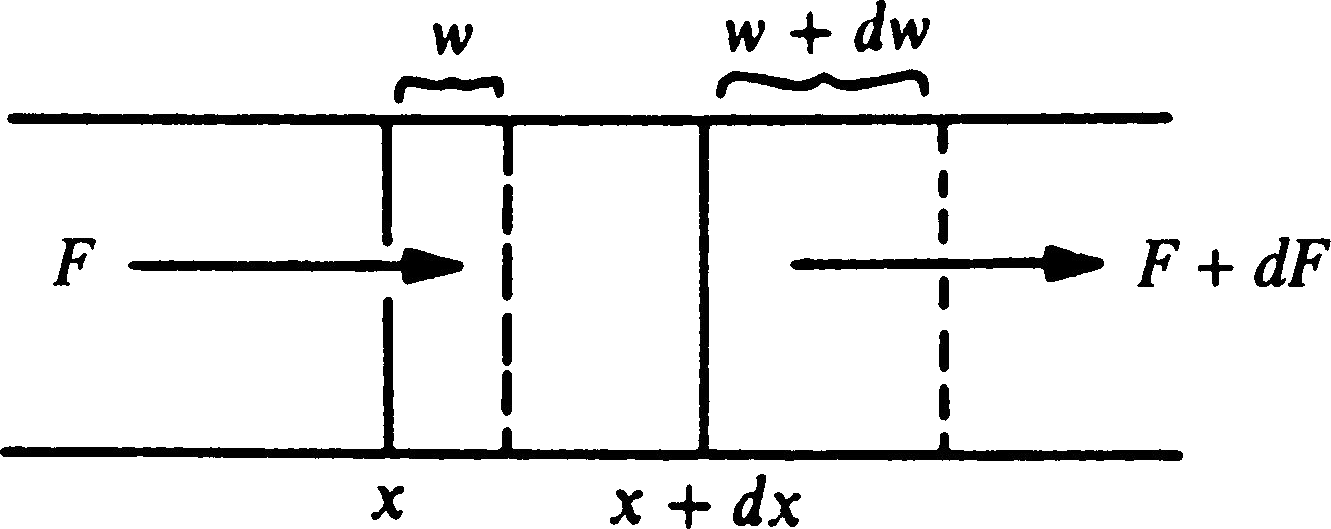
\includegraphics[width=0.55\linewidth]{00_Images/02_chapter/10.png}
    \caption{Forces and displacement of a differential bar element in longitudinal motion}
    \label{fig:bar_element_longitudinal}
\end{figure}

Consider a short bar element of length \( dx \), cross-sectional area \( S \), density \( \rho \)  and Young modulus \( E \) (figure \ref{fig:bar_element_longitudinal}). Let \( w(x,t) \) be the longitudinal displacement of the cross section at position \( x \). The longitudinal strain is
\[
\varepsilon(x,t) = \frac{\partial w}{\partial x}
\]
and Hooke's law relates stress and strain as \( \sigma = E\varepsilon \). Since \( \sigma = F/S \), one obtains
\[
F(x,t) = SE\frac{\partial w}{\partial x}
\]
Expanding \( F(x + dx,t) \) to first order gives
\[
dF = F(x + dx,t)-F(x,t) = \frac{\partial F}{\partial x}dx
   = SE\frac{\partial^2 w}{\partial x^2}dx
\]
The mass of the element is \( \rho Sdx \), hence Newton's law yields
\[
dF = \rho Sdx\frac{\partial^2 w}{\partial t^2}
\]
Combining the two relations gives the 1D longitudinal wave equation
\[
\frac{\partial^2 w}{\partial t^2}
 = 
\frac{E}{\rho}\frac{\partial^2 w}{\partial x^2}
\]
with longitudinal wave speed
\[
c_L = \sqrt{\frac{E}{\rho}}
\]
The structure of this equation is identical to the transverse-string wave equation, but the wave speed is now set by material parameters, not by tension. As a consequence, longitudinal waves also exist in stiff strings and their resonance frequencies are generally not in harmonic relation with the transverse ones. 

\paragraph{Mode frequencies} For a bar of length \( L \), the end conditions determine the standing waves. In particular:
\[
f_n = \frac{nc_L}{2L},\qquad n = 1,2,3,\dots
\]
for both ends fixed or both ends free, while for a bar fixed at one end and free at the other,
\[
f_m = \frac{mc_L}{4L},\qquad m = 1,3,5,\dots
\]
as in the standard quarter-wave pattern.

\subsection{Bending Waves in a Thin Bar (Flexural Waves)}

Bars also support transverse motion \( y(x,t) \) due to bending. In the thin-bar (Euler-Bernoulli) approximation, the transverse dynamics are governed by a fourth-order PDE, which may be written as
\[
\frac{\partial^2 y}{\partial t^2}
 = 
-\frac{E K^2}{\rho}\frac{\partial^4 y}{\partial x^4}
\]
Here \( K \) is the radius of gyration of the cross section,
\[
K^2 = \frac{1}{S}\int z^2dS
\]
where \( z \) is the distance from the neutral axis and \( S \) is the cross-sectional area. Figure \ref{fig:gyration_radius} illustrates the radius of gyration for typical cross-sectional shapes.

\begin{figure}[!htb]
    \centering
    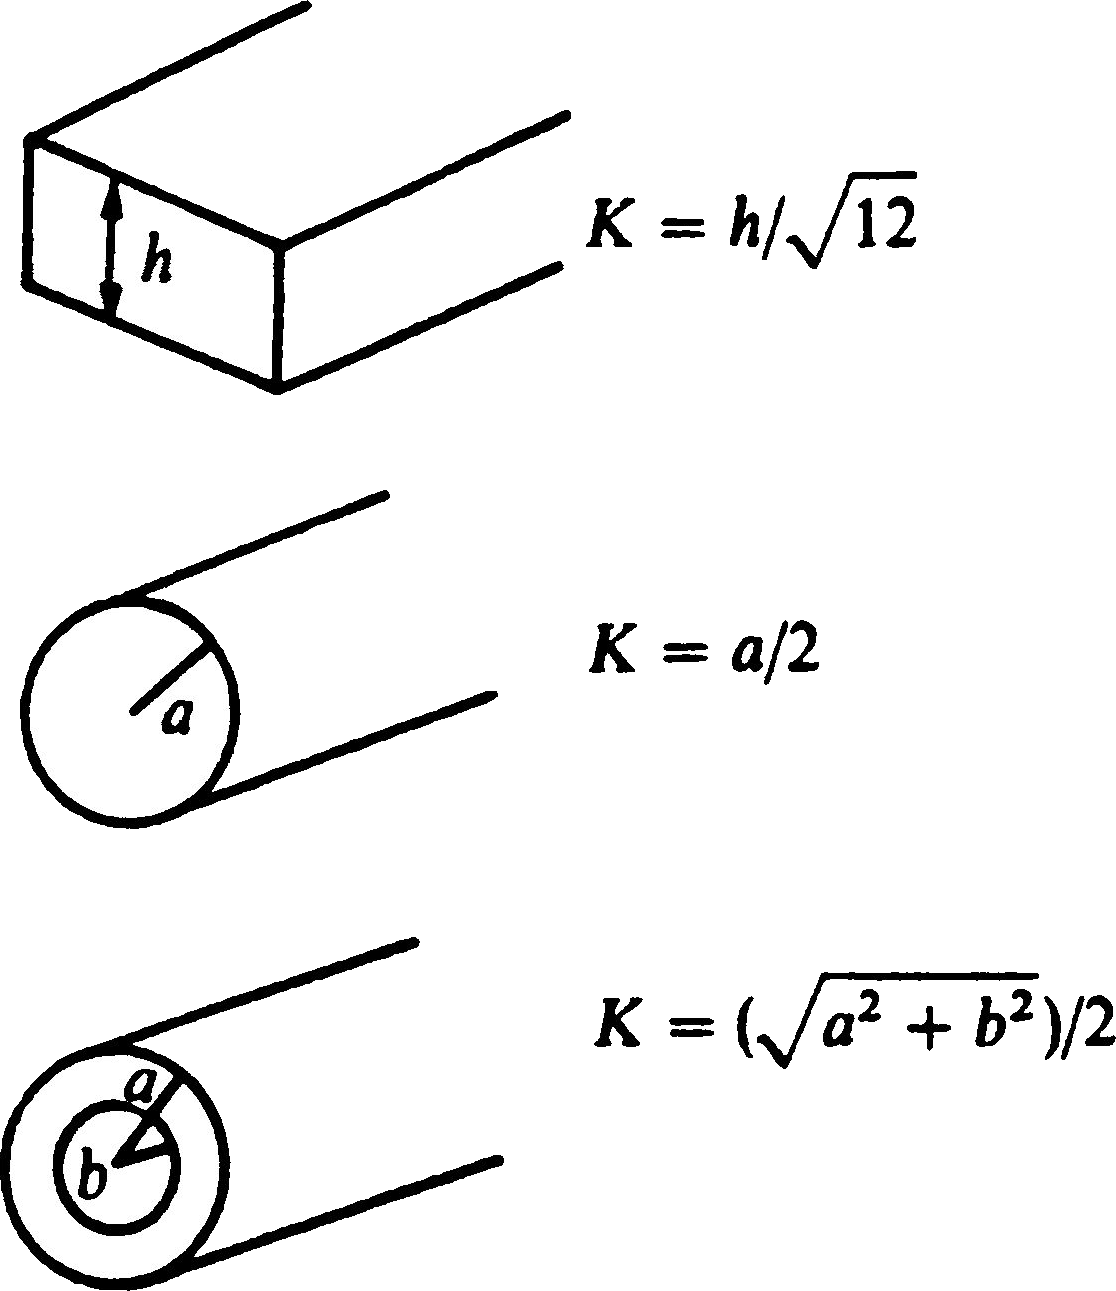
\includegraphics[width=0.5\linewidth]{00_Images/02_chapter/11.png}
    \caption{Radius of gyration \(K\) for typical bar cross sections}
    \label{fig:gyration_radius}
\end{figure}

\paragraph{Dispersion and propagation number} Because a fourth spatial derivative appears, flexural waves are dispersive: different frequency components propagate at different speeds. Introducing a separable harmonic solution
\[
y_e(x,t) = Y_e(x)e^{-j\omega t}
\]
and substituting gives
\[
\frac{d^4 Y_e}{dx^4} = \frac{\rho\omega^2}{E K^2}Y_e
\]
Defining the propagation number \( k \) through
\[
k^4 = \frac{\rho\omega^2}{E K^2}
\]
one finds the dispersion relation
\[
\omega = K\sqrt{\frac{E}{\rho}}k^2
\qquad
v_p = \frac{\omega}{k}
 = \left(K\sqrt{\frac{E}{\rho}}\right)k
\propto \sqrt{\omega}
\]
so the phase speed increases with frequency. 

\paragraph{General harmonic solution} Seeking exponential solutions \( Y_e(x) = Ae^{\gamma x} \) gives \( \gamma^4 = k^4 \), hence
\[
\gamma = \pm k,\qquad \gamma = \pm jk
\]
Therefore, the general harmonic motion in a thin bar can be written as
\[
y_e(x,t) = e^{j\omega t}\left(Ae^{kx} + Be^{-kx} + Ce^{jkx} + De^{-jkx}\right)
\]
and the constants are determined by the boundary conditions at the ends.

\subsection{End Supports and Modal Frequencies in a Thin Bar}

For flexural motion, endpoint conditions involve both displacement and derivatives, because bending moment and shear force depend on curvature and its derivative. Three idealized supports are commonly used:

\begin{itemize}
\item Free end: no bending moment and no shear force,
\[
\left.\frac{\partial^2 y}{\partial x^2}\right|_{\text{end}} = 0,
\qquad
\left.\frac{\partial^3 y}{\partial x^3}\right|_{\text{end}} = 0.
\]
\item Supported end (simply supported): zero displacement and no bending moment,
\[
\left.y\right|_{\text{end}} = 0,
\qquad
\left.\frac{\partial^2 y}{\partial x^2}\right|_{\text{end}} = 0.
\]
\item Clamped end: zero displacement and zero slope,
\[
\left.y\right|_{\text{end}} = 0,
\qquad
\left.\frac{\partial y}{\partial x}\right|_{\text{end}} = 0.
\]
\end{itemize}

Figure \ref{fig:diffendbar} summarizes what is written above and figure \ref{fig:barmodeshapes} shows the corresponding normal-mode shapes and relative modal frequencies for the most common end conditions described after.

\begin{figure}[!htb]
    \centering
    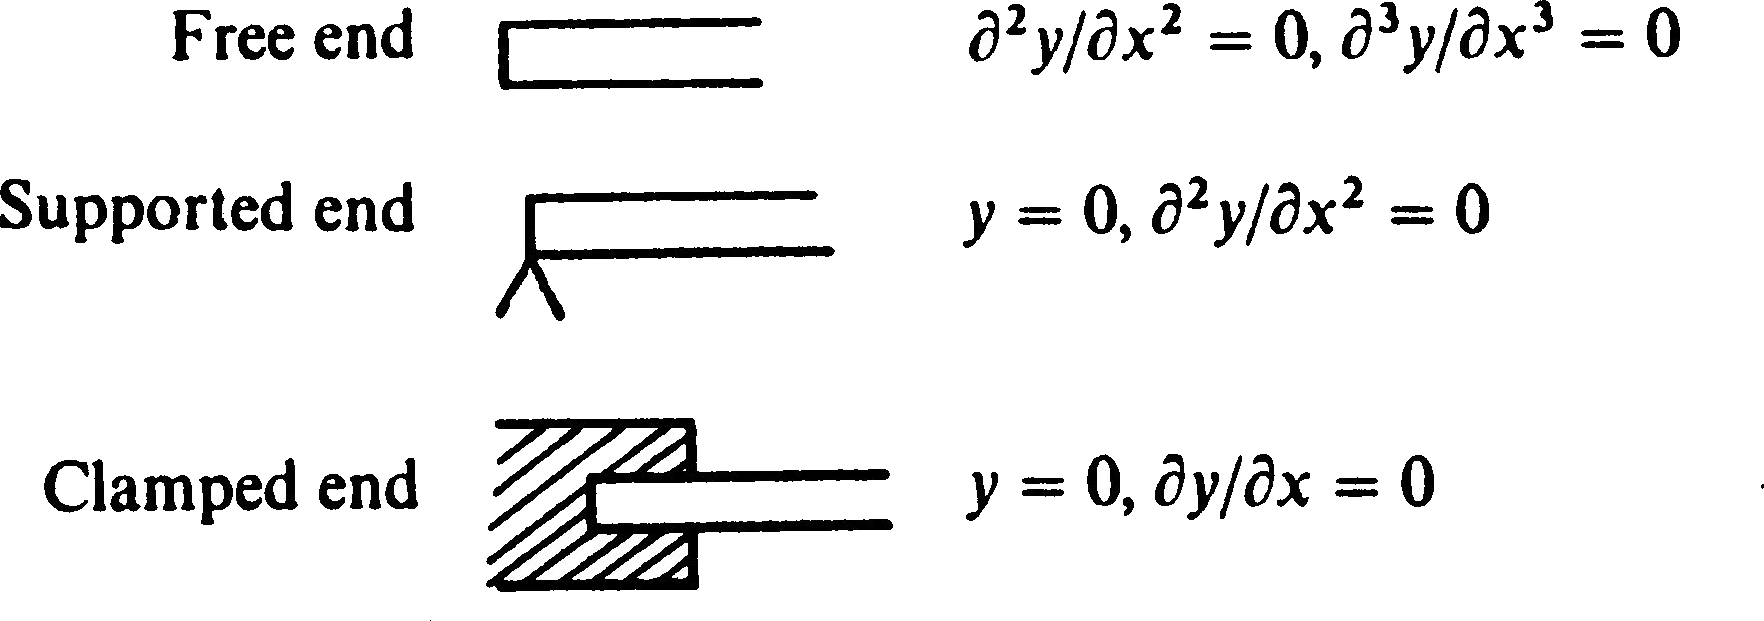
\includegraphics[width=0.65\linewidth]{00_Images/02_chapter/12.png}
    \caption{Idealized boundary conditions for flexural vibration: free, simply supported, and clamped ends}
    \label{fig:diffendbar}
\end{figure}

\begin{figure}[!htb]
    \centering
    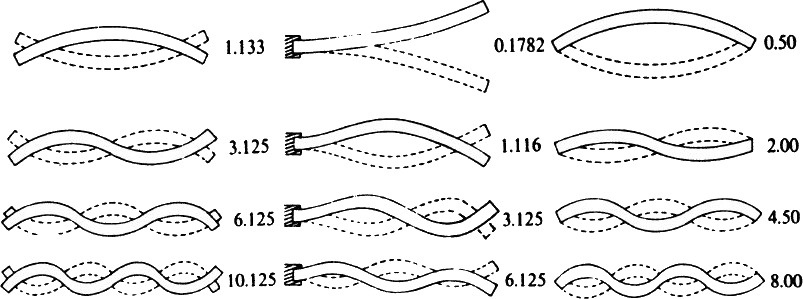
\includegraphics[width=0.85\linewidth]{00_Images/02_chapter/13.png}
    \caption{Normal modes of a bar for typical end conditions and their relative frequencies}
    \label{fig:barmodeshapes}
\end{figure}


\paragraph{Free-free bar} For a bar of length \( L \) free at both ends, the boundary conditions lead to the transcendental equation
\[
\tan\left(\frac{kL}{2}\right) = \pm\tanh\left(\frac{kL}{2}\right)
\]
whose roots yield the flexural modal frequencies in the form
\[
f_n = \frac{\pi K}{8L^2}\sqrt{\frac{E}{\rho}}
\beta_n^2,
\qquad
\beta_n\approx \left[3.011, 5, 7,\dots,(2n + 1)\right]
\]
The spacing is not harmonic and the departure from harmonicity is a direct consequence of dispersion.

\paragraph{Clamped-free bar (cantilever)} For a cantilevered bar (clamped at \( x = 0 \), free at \( x = L \) ), the characteristic condition becomes
\[
\cot\left(\frac{kL}{2}\right) = \pm\tanh\left(\frac{kL}{2}\right)
\]
leading to
\[
f_n = \frac{\pi K}{8L^2}\sqrt{\frac{E}{\rho}}
\beta_n^2,
\qquad
\beta_n\approx \left[1.1194, 2.988, 5, 7, \dots, (2n-1)\right]
\]
with frequencies lower than the free-free case. 

\paragraph{Supported-supported bar} For a bar supported at both ends, the modal frequencies reduce to the simple quadratic law
\[
f_m = \frac{\pi K}{2L^2}\sqrt{\frac{E}{\rho}}m^2,
\qquad
m = 1,2,3,\dots
\]
again emphasizing the non-harmonic pattern typical of flexural modes.

\section{Vibrations in Stiff Strings}

The ideal string model assumes that the restoring force is provided only by the string tension. In many practical cases (notably metallic strings), stiffness is not negligible and contributes an additional restoring action. The resulting dynamics combine the tension-driven wave equation with a bending (flexural) term, so the string becomes dispersive and its partials are no longer exactly harmonic.

\subsection{Equation of Motion and Dispersion Relation}

Let \( y(x,t) \) be the transverse displacement, \( T \) the tension and \( \mu \) the linear mass density. Including stiffness effects leads to the modified PDE
\[
\frac{\partial^{2}y}{\partial t^{2}}
 = 
c^{2}\frac{\partial^{2}y}{\partial x^{2}}
-\frac{ESK^{2}}{\mu}\frac{\partial^{4}y}{\partial x^{4}}
\]
where \( E \) is Young's modulus, \( S \) is the cross-sectional area and \( K \) is the radius of gyration of the cross section. Although does not generally admit a simple closed-form solution, useful insight follows from a traveling-wave ansatz
\[
y(x,t) = e^{j(\omega t-kx)}
\]
Substitution yields the dispersion equation
\[
\omega^{2} = k^{2}c^{2}\left(1 + \frac{EI}{T}k^{2}\right)
\]
where \( I \) is the second moment of area of the cross section. In particular, higher \( k \) (shorter wavelength) components have larger phase speed, which is the hallmark of dispersion, hence waveforms deform as they propagate.

\subsection{Normal Modes and Inharmonicity}

Introducing the dimensionless parameter
\[
\epsilon = \frac{EI}{TL^{2}}
\]
the dispersion relation may be rewritten as
\[
\omega^{2} = k^{2}c^{2}\left(1 + \epsilon k^{2}L^{2}\right)
\]
For a stiff string with supported (hinged) ends, the displacement and bending moment vanish at \( x = 0 \) and \( x = L \), leading to the wavenumber condition
\[
\sin(kL) = 0
\quad\Longleftrightarrow\quad
k_nL = n\pi
\]
The corresponding natural frequencies can be expressed as
\[
f_n = n f_1^{\circ}\sqrt{1 + Bn^{2}},
\qquad
B = \frac{\pi ESK^{2}}{TL^{2}}
\]
where \( f_1^{\circ} \) is the fundamental frequency of the same string in the ideal (tension-only) model. 

\paragraph{Discussion} The factor \( \sqrt{1 + Bn^{2}} \) shows that stiffness increases the frequencies with respect to the ideal string and the effect grows with mode number \( n \): high partials are stretched upward. Consequently, the partials are not in an exact harmonic relationship with the fundamental.

\subsection{Clamped Ends and Further Frequency Shifts}

If the ends are clamped rather than supported, the natural frequencies are further increased. A commonly used approximation is
\[
f_n
 = 
n f_1^{\circ}\sqrt{1 + Bn^{2}\left[1 + \frac{2}{\pi}B^{1/2} + \left(\frac{4}{\pi^{2}}\right)B\right]}
\]
In this case the end constraints stiffen the boundary, raising the modal frequencies. The stretching of the partials is present but may be slightly reduced in relative terms compared to the supported-end case. 

\subsection{Relevant Musical Cases}

\paragraph{Piano strings} For the lower piano strings, stiffness would cause overtones to deviate from harmonic tuning with the fundamentals of the upper strings. In practice, tuning compensates by stretching octaves slightly above the ideal \( 2:1 \) ratio. For example, the 4th harmonic of C4 may be a few cents sharp and the same harmonic for C5 even more so.

\paragraph{Violin strings} Metal violin strings also exhibit non-negligible stiffness. Dispersion implies that sharp bends in the bowed-string waveform do not propagate rigidly: the corner is sharp near the bow position but becomes progressively rounded while it travels freely, until it reaches the bow again.

\section{Dispersion: Phase and Group Velocity}

For an ideal (tension-only) string, the dispersion relation is linear,
\[
\omega = ck,
\qquad c = \sqrt{\frac{T}{\mu}}
\]
so all frequency components propagate with the same speed and a traveling waveform preserves its shape. Whenever the relation \( \omega(k) \) is not a straight line, the medium is dispersive: different wavenumbers travel differently and waveforms deform as they propagate. Two important cases in musical acoustics are stiff strings and strings loaded with discrete masses. Representative dispersion relations for these cases are compared in figure \ref{fig:dispersion_examples}.

\begin{figure}[!htb]
    \centering
    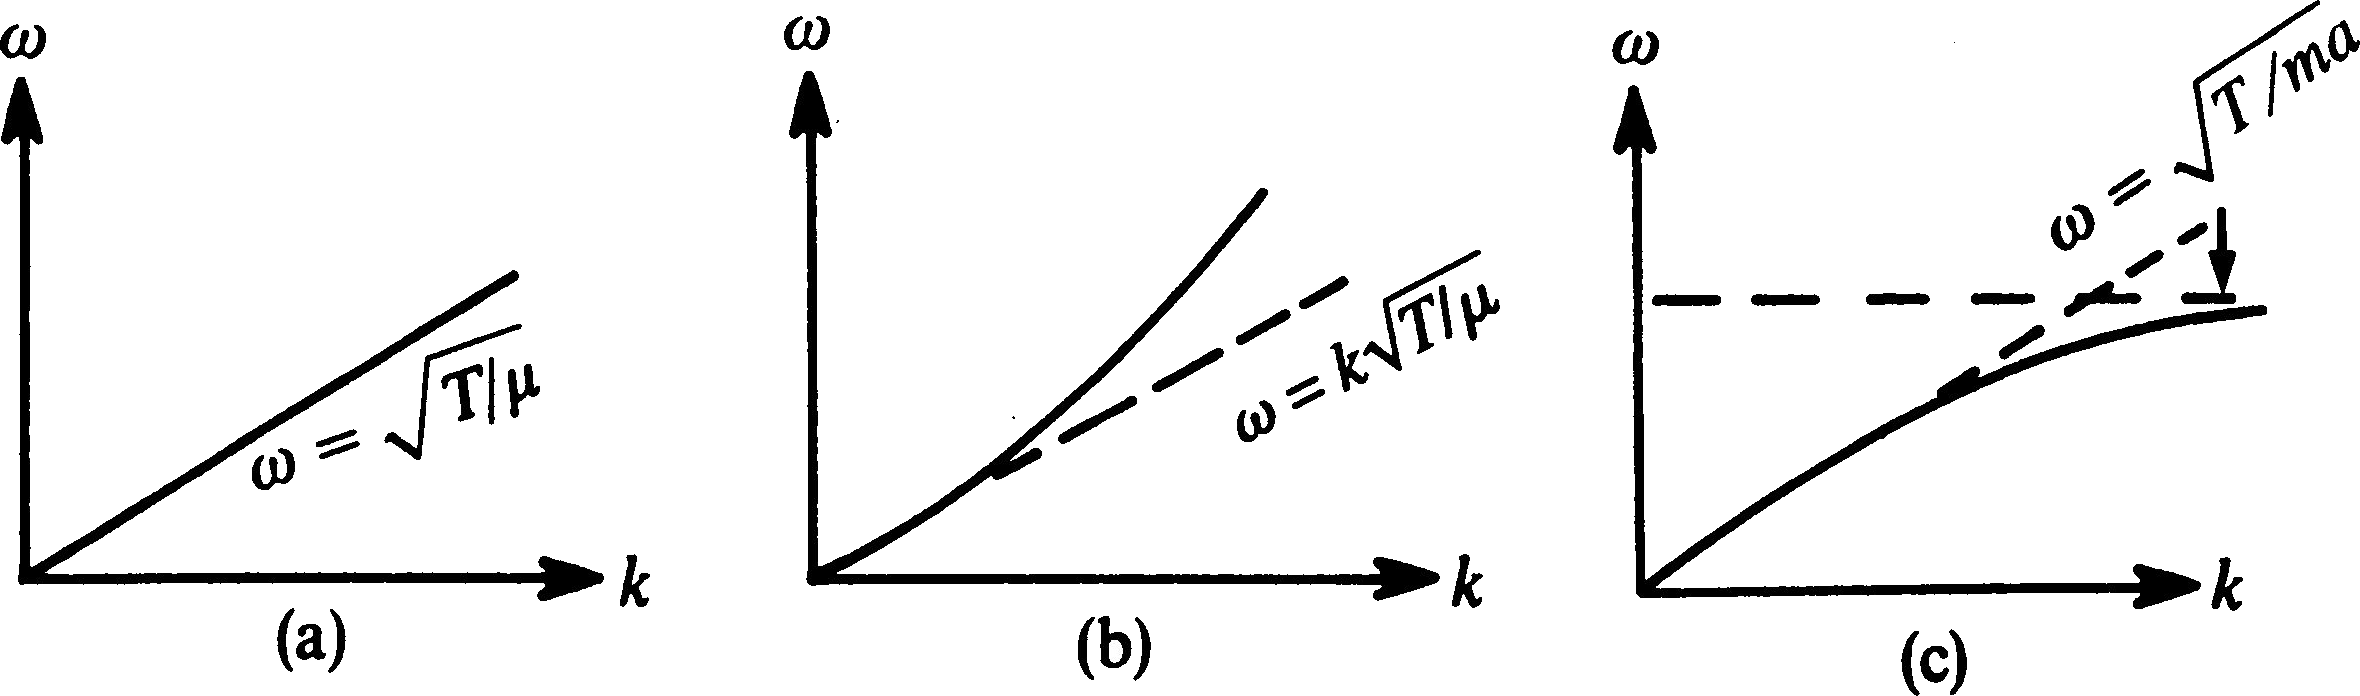
\includegraphics[width=0.9\linewidth]{00_Images/02_chapter/14.png}
    \caption{Dispersion relations for ideal, stiff, and mass-loaded strings}
    \label{fig:dispersion_examples}
\end{figure}

\subsection{Dispersion in Stiff Strings}

For a string with non-negligible stiffness (hinged ends), the natural frequencies can be expressed as
\[
\omega_n
 = 
n k_s \sqrt{\frac{T}{\mu}}\sqrt{1 + Bn^{2}}
 = 
n k_s \sqrt{\frac{T}{\mu}}\sqrt{1 + \alpha k^{2}}
\]
showing explicitly that the dependence on \( k \) (or on mode number \( n \) ) is no longer linear. As a consequence, higher partials propagate with a different effective velocity and the modal frequencies deviate from exact harmonicity. 

\subsection{String Loaded with Equally Spaced Masses and Cutoff Frequency}

Consider now a string loaded with identical masses \( m \) (``beads'') equally spaced by a distance \( a \). In this case a different type of dispersion arises, with dispersion relationship
\[
\omega(k) = 2\sqrt{\frac{T}{ma}}\sin(ka),
\qquad 0\le k \le \frac{\pi}{a}
\]
The allowed values of \( k \) between \( 0 \) and \( \pi/a \) equal the number of normal modes of the system, which is also equal to the number of masses. The maximum value of \( \omega \) is
\[
\omega_{\max} = 2\sqrt{\frac{T}{ma}}
\quad (\text{attained at } k = \pi/a)
\]
and the corresponding cutoff frequency is defined as
\[
f_c = \frac{\omega_{\max}}{2\pi}
 = 
\frac{1}{\pi}\sqrt{\frac{T}{ma}}
\]
It represents the highest frequency of a wave disturbance that can propagate on the loaded string. Moreover, at \( k = \pi/a \) the group velocity vanishes, meaning that energy transport stops even though a phase can still be defined.

\paragraph{Phase and group velocity} From the graph of \( \omega \) versus \( k \) (ideal string: straight line; dispersive cases: curved line), two different velocities are defined:
\[
v_\phi = \frac{\omega}{k},
\qquad
v_g = \frac{d\omega}{dk}
\]
The phase velocity \( v_\phi \) is the velocity of a wave crest (or any fixed phase), while the group velocity \( v_g \) is the velocity of the wave envelope (wave packet) and therefore it governs energy transport. In dispersive media, \( v_\phi\neq v_g \) in general. 

\section{Torsional Vibrations in a Bar}

Besides transverse and longitudinal motion, a slender bar (and, to some extent, a string) can also sustain torsional waves, i.e. waves of angular twist about the longitudinal axis. The governing equation is obtained by equating the net torque acting on an infinitesimal element to the product of its polar moment of inertia and its angular acceleration. The resulting PDE has the same mathematical form as the longitudinal wave equation and, importantly, torsional waves are nondispersive: their propagation velocity is independent of frequency. 

\subsection{Wave Equation and Propagation Speed}

Let \( \theta(x,t) \) denote the twist angle. For a uniform bar made of a material with shear modulus \( G \) and density \( \rho \), the torsional wave speed is
\[
c_t = \sqrt{\frac{G K_T}{\rho I}}
\]
where \( I \) is the polar moment of inertia (per unit length in the 1D model) and \( K_T \) is a torsional stiffness factor that accounts for the cross-section shape (it relates twist to the shear strain produced). A useful relation connects \( G \) to Young's modulus \( E \) and Poisson's ratio \( \nu \):
\[
G = \frac{E}{2(1 + \nu)}
\]
Poisson's ratio measures the lateral contraction under an axial traction (Poisson effect).

\paragraph{Dependence on cross-section} For a circular rod one has \( K_T = I \), hence
\[
c_t = \sqrt{\frac{G}{\rho}}
\]
For non-circular cross sections the speed is slightly reduced. Typical approximations reported are
\[
c_t \simeq 0.92\sqrt{\frac{G}{\rho}} \quad \text{(square)},
\quad
c_t \simeq 0.74\sqrt{\frac{G}{\rho}} \quad \text{(rectangular}),
\quad
c_t \simeq \frac{2h}{w}\sqrt{\frac{G}{\rho}} \quad (w > 6h)
\]

\begin{figure}[!htb]
    \centering
    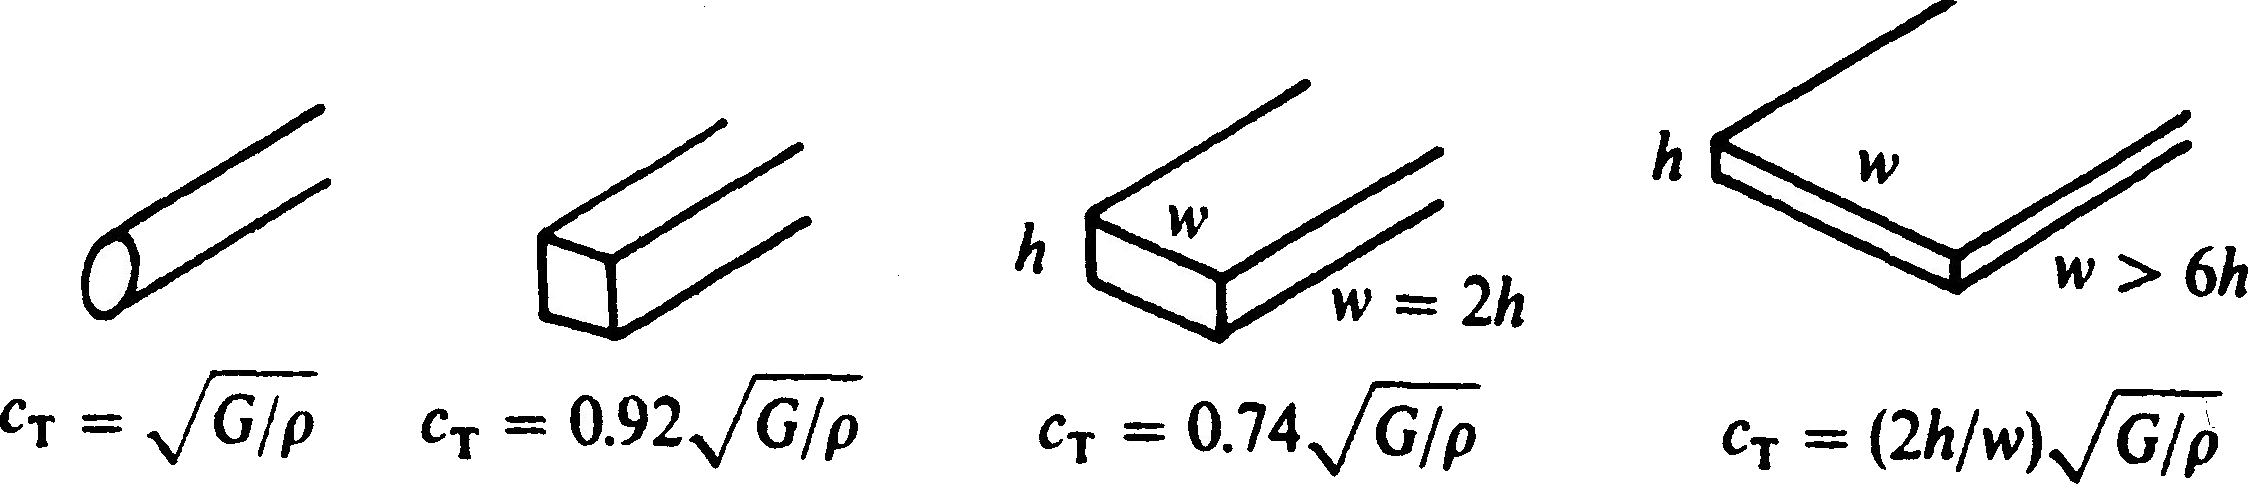
\includegraphics[width=0.9\linewidth]{00_Images/02_chapter/15.png}
    \caption{Torsional wave speed for different bar cross sections}
    \label{fig:torsion_speed_sections}
\end{figure}

\subsection{Standing Waves and Torsional Mode Frequencies}

For a bar of length \( L \), torsional modes follow directly from the nondispersive relation \( \omega = c_t k \). For free-free (or fixed-fixed) ends, the allowed wavenumbers are
\[
k_n = \frac{n\pi}{L},\qquad n = 1,2,3,\dots
\]
leading to the torsional modal frequencies
\[
f_n = \frac{\omega_n}{2\pi} = \frac{n c_t}{2L}
\]
If one end is clamped and the other is free, the quarter-wave condition applies and only odd indices occur,
\[
f_m = \frac{m c_t}{4L},\qquad m = 1,3,5,\dots
\]
in direct analogy with longitudinal modes. 

\paragraph{Torsion in bowed strings} Bowing a violin string excites torsional waves as well as transverse waves. A key point is that \( c_t \) is typically larger than the transverse wave speed \( c \), with reported ratios \( c_t/c \) ranging roughly from \( 2 \) up to \( 7.6 \) depending on string type and construction. The damping of torsional waves (reported around 1\% to 7\%) is dominated by internal damping rather than reflection losses at the bridge and nut and torsional motion affects the effective compliance of the string and the bow-string interaction.

\section{Nonlinear Effects in Strings}

The linear string model assumes that the vibration amplitude is proportional to the excitation amplitude. Whenever this proportionality fails, the behavior is nonlinear. In strings, two broad mechanisms can produce nonlinearity: material effects (elastic moduli depending on strain) and geometric effects. Here we focus on the second mechanism, which becomes relevant when transverse displacements are large.

\subsection{Geometric Nonlinearity: Length Change and Tension Modulation}

Consider the vibration dominated by a single mode \( n \), written (for simplicity) as
\[
y_n(x,t) = a_n\sin\left(\frac{n\pi x}{L}\right)\cos(\omega_n t),
\qquad
\omega_n = \frac{n\pi}{L}\sqrt{\frac{T}{\rho S}}
\]
where \( T \) is the (nominal) tension, \( S \) the cross-sectional area and \( \rho S \) the mass per unit length. Because the string is not perfectly inextensible, transverse motion produces a (second-order) increase of its arc length. The instantaneous length is
\[
L(t) = \int_{0}^{L}\left[1 + \left(\frac{\partial y}{\partial x}\right)^2\right]^{1/2}dx
\]
hence the length variation is
\[
\delta L(t) = L(t)-L
\simeq
\frac{n^{2}\pi^{2}a_n^{2}}{8L}\left(1-\cos 2\omega_n t\right)
\]
This expression contains a steady term and an oscillating term at frequency \( 2\omega_n \). The corresponding tension variation follows from the axial stiffness of the string:
\[
\delta T(t) = \frac{ES}{L}\delta L(t)
 = 
\overline{\delta T} + \Delta T_n\cos(2\omega_n t)
\]
where \( E \) is Young's modulus, \( \overline{\delta T} \) is the steady increase in tension and \( \Delta T_n \) is the amplitude of the oscillating component.

\subsection{Consequences}

\paragraph{Inharmonicity from time-varying tension} Since (in the linear model) modal frequencies scale as \( \omega_n\propto \sqrt{T} \), a small tension modulation produces
\[
\omega_n(t)
 = 
\omega_n\sqrt{1 + \frac{\delta T(t)}{T}}
\simeq
\omega_n\left[1 + \frac{1}{2}\frac{\overline{\delta T}}{T}
 + \frac{1}{2}\frac{\Delta T_n}{T}\cos(2\omega_n t)\right]
\]
The steady term shifts all frequencies upward, while the oscillating term produces a time-varying detuning. Because the magnitude of \( \Delta T_n \) depends on the mode and on the vibration amplitude, different harmonics are affected differently: harmonicity is progressively destroyed until the vibration decays to a sufficiently small level.

\paragraph{Possible countermeasures} Geometric nonlinearity is reduced by using longer strings or with smaller \( E \) or tuned with higher tension \( T \).

\paragraph{Appearance of new modal components} The tension modulation at \( 2\omega_n \) acts as a parametric perturbation. In an ideally clamped string, the oscillating term does not primarily generate components at \( 2\omega_n \), but rather leads to contributions around \( 3\omega_n \). When the termination (bridge) is not perfectly rigid, vibrations near \( 3\omega_n \) can couple into spatial modes and generate the mode \( 2n \). In practice, this effect may be masked when other sources already create spurious oscillations.

\paragraph{Precession of the polarization} Real string motion is generally not confined to a single transverse plane: an oscillation polarized in the \( (x,y) \) plane may coexist with (and excite) an oscillation in the orthogonal \( (x,z) \) plane. The geometric nonlinearity generates components at \( 2\omega_n \) that can set the bridge into motion, providing a forcing path between the two polarizations. As a result, energy is transferred between the two planes and the vibration ellipse precesses. A characteristic rate for this exchange is commonly written as
\[
\Omega = A\frac{ES}{T}\frac{ab}{L^{2}}\omega
\]
where \( A \) is close to unity, \( a \) and \( b \) are the minor and major axes of the polarization ellipse and \( \omega \) is the oscillation frequency. Typical precession time scales are of the order of 1 s and the rate decreases as the vibration amplitude decays.
